\documentclass[a4paper]{article}
\usepackage[right=1in, left=1in, top=1in, bottom=1in]{geometry}
\usepackage{graphicx}
\begin{document}
	\title{\textbf{MACHINE LEARNING LAB}}
	\maketitle
	\centering{\textbf{Manish Singh CS3}}\\
	\centering{\textbf{Roll No. 17/466}}\\
	\begin{figure}[h]
		\centering
		
\includegraphics{rtu.jpeg}
	\end{figure}\\

	\begin{large}
		Computer Science and Engineering Department
	\end{large}\\
\newline
	\begin{Large}
			Rajasthan Technical University, Kota\\[2.5]\\
	\end{Large}
	\newpage
	\flushleft
	\tableofcontents
	\newpage
	\section{Problem Statement}
		For a given set of training data examples stored in a .CSV file, implement and demonstrate the Candidate Elimination algorithm to output a description of the set of all hypotheses consistent with the training examples.(enjoysport.csv)\\
	\section{Candidate Elimination algorithm}
	1. Initialize $h$ to the most specific hypothesis in $S$\\
    2. Initialize $h$ to the most General hypothesis in $G$\\
    3. For each example in data set\\
	\hspace{10mm}If ( $e$ is a positive example) then\\
	\hspace{20mm}Elements of $G$ that classify $e$ as negative are removed from $G$\\
	\hspace{20mm}Each element $s$ of $S$ that classifies $e$ as negative is removed and replaced by the minimal \\
	\hspace{20mm}generalizations of $s$ that classify $e$ as positive and are less general than some member of $G$\\
	\hspace{30mm}Non-maximal hypotheses are removed from $S$;\\
	\hspace{10mm}Else    Elements of $S$ that classify $e$ as positive are removed from $S$\\
	\hspace{20mm}Each element $g$ of $G$ that classifies $e$ as positive is removed and replaced by the minimal \\
	\hspace{20mm}specializations of $g$ that classifies $e$ as negative and are more general than some member of \\ \hspace{20mm}$S$\\
	\hspace{30mm}Non-minimal hypotheses are removed from $G$ \\
	
	
	\section{Training Set}
	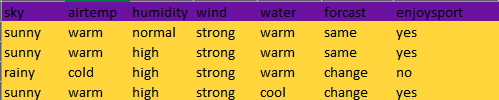
\includegraphics[scale=1.3]{enjoysport.png}
	\newpage
	\section{Program}
	\begin{verbatim}
	import numpy as np
	import pandas as pd
	
	data = pd.DataFrame(pd.read_csv('enjoysport.csv'))
	concepts = np.array(data.iloc[:,:-1])
	target = np.array(data.iloc[:,-1])
	
	def learn(concepts, target):
	specific_h = concepts[0].copy()
	general_h = [["?" for i in range(len(specific_h))] for i in range(len(specific_h))]
	
	for i, h in enumerate(concepts):                
	if target[i] == "yes":
	for x in range(len(specific_h)):
	if h[x] != specific_h[x]:
	specific_h[x] = '?'
	general_h[x][x] = '?'
	print(" \n\nFor Training instance No:{0} the hypothesis is\n".format(i))
	print("Specific Hypothesis: ",specific_h)
	print("General Hypothesis: ",general_h,)
	if target[i] == "no":            
	for x in range(len(specific_h)):
	if h[x] != specific_h[x]:
	general_h[x][x] = specific_h[x]
	else:
	general_h[x][x] = '?'
	print(" \n\nFor Training instance No:{0} the hypothesis is\n".format(i))
	print("Specific Hypothesis: ", specific_h)
	print("General Hypothesis: ",general_h,)
	indices = [i for i,val in enumerate(general_h) if val == ['?', '?', '?', '?', '?', '?']]
	
	for i in indices:
	general_h.remove(['?', '?', '?', '?', '?', '?'])
	
	return specific_h, general_h
	print("*"*20,"Costumer Elimination Algorithm","*"*20)
	s_final, g_final = learn(concepts, target)
	print("Final Specific hypothesis:", s_final)
	print("Final General hypothesis:", g_final)
	\end{verbatim}
	\section{Output}
	\fbox{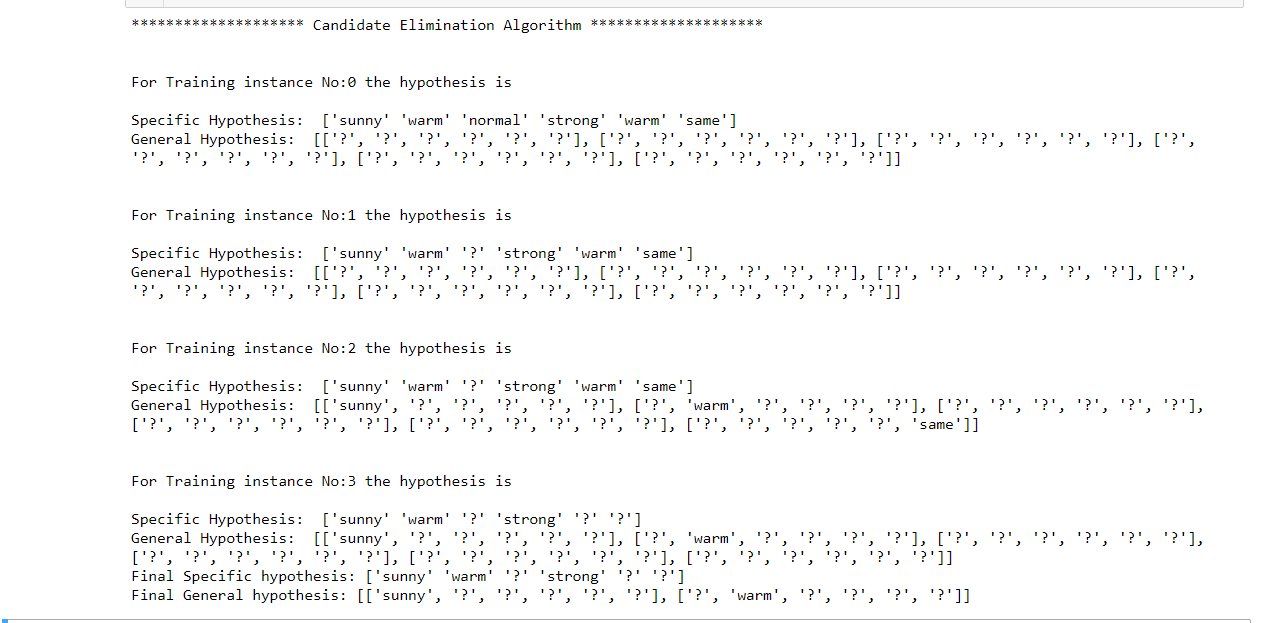
\includegraphics[scale=1.0]{candidate.png}}
	\section{Result}
	We have found the most specific hypothesis and most genral hypothesis based on a given set of training data samples using Candidate Elimination algorithm.
\end{document}